\documentclass[10pt,twocolumn]{article}

\usepackage[T1]{fontenc}
\usepackage[utf8]{inputenc}
\usepackage{mathptmx}
\usepackage[margin=0.72in,columnsep=0.24in]{geometry}
\usepackage{microtype}
\usepackage{graphicx}
\usepackage{booktabs}
\usepackage{amsmath}
\usepackage{array}
\usepackage[numbers,sort&compress]{natbib}
\usepackage[hidelinks]{hyperref}
\hypersetup{
  pdftitle={Matched-Recovery Benchmarking of Ocular Activation Codes in Spontaneous REM Sleep},
  pdfauthor={Javier Emilio Bazan Sanchez}
}

\setlength{\parindent}{1em}
\setlength{\parskip}{0pt}
\setlength{\textfloatsep}{8pt plus 2pt minus 2pt}
\setlength{\floatsep}{7pt plus 2pt minus 2pt}
\setlength{\intextsep}{7pt plus 2pt minus 2pt}
\renewcommand{\arraystretch}{1.08}

\title{\vspace{-1.1em}\textbf{Matched-Recovery Benchmarking of Ocular Activation Codes in Spontaneous REM Sleep}\vspace{-0.4em}}
\author{Javier Emilio Bazan Sanchez\\
\small Facultad de Ciencias, Universidad Nacional Aut\'onoma de M\'exico\\
\small \href{mailto:bazan@ciencias.unam.mx}{bazan@ciencias.unam.mx}}
\date{}

\begin{document}
\maketitle

\begin{abstract}
Voluntary eye movements allow a person in a lucid dream to send simple signals from verified rapid eye movement (REM) sleep. A practical interface must distinguish those signals from the eye movements that occur naturally during REM. This study tested whether a rhythmic eight-interval code was less likely to appear by chance than an equal-duration, evenly timed code. Both codes were scanned continuously in expert-scored REM electrooculography from Sleep-EDF Expanded. Detection thresholds were chosen separately so that the codes recovered the same proportion of paired synthetic signals. The primary sleep-cassette study included 129 nights from 66 participants and 177.13 eligible REM hours. At 90\% matched synthetic recovery, the rhythmic code produced 1.823 detections per hour and the control produced 1.694, a difference of 0.130 per hour (95\% interval after resampling participants: $-1.149$ to 1.102). A separately frozen replication used 22 placebo nights from 22 sleep-telemetry participants and 34.24 eligible REM hours. At 95\% matched recovery, rates were 8.996 and 9.376 per hour, a difference of $-0.380$ (95\% interval: $-10.523$ to 12.394). Neither study supported lower collision for the rhythmic code. Applying thresholds from the first corpus directly to the second created a much larger apparent advantage, but the two codes then had unequal recovery. The results show why continuous-time, exposure-normalized, equal-recovery evaluation is necessary before an ocular code is used as an asynchronous dream interface.
\end{abstract}

\section{Introduction}

People can sometimes recognize that they are dreaming while the dream continues. In laboratory studies, lucid dreamers have marked this state with prearranged left-right eye movements recorded in the electrooculogram (EOG) during polysomnographically verified REM sleep \citep{laberge1981}. The same channel has supported time-stamping of dream tasks \citep{laberge2018} and, more recently, real-time question answering through eye or facial-muscle responses \citep{konkoly2021}. These findings establish ordinary sensory input and physiological output during sleep. They do not imply telepathy or anomalous information transfer.

The engineering problem is less settled. An asynchronous interface must monitor a continuous signal and activate only when the intended code occurs. Short ocular patterns can also arise during spontaneous REM. Voss and colleagues reported frequent accidental matches to a short left-right-left pattern and used longer, separated sequences to improve identification \citep{voss2009}. Later work used template matching for successive left-right signals, followed by expert validation \citep{laberge2018}. Outside sleep, continuous EOG interfaces likewise treat false activations per unit time as a central design constraint \citep{wang2014,fang2018}.

This study evaluates that constraint directly. A rhythmic eight-interval candidate was compared with an isochronous control of equal nominal duration. The unit of performance was not window accuracy. It was the number of accidental detections per eligible hour of spontaneous, expert-scored REM sleep at equal recovery of prespecified synthetic engineering signals. A large sleep-cassette cohort provided the primary test. A second sleep-telemetry cohort provided an external, separately frozen test of a high-recovery pattern suggested by the first study.

\section{Methods}

\subsection{Study design and data}

Both analyses used the public Sleep-EDF Expanded database on PhysioNet \citep{kemp2000,goldberger2000}. The horizontal EOG was sampled at 100 Hz. Expert hypnograms defined REM exposure. Two seconds were removed from each REM boundary, and samples affected by nonfinite values or sustained flatlines were excluded by fixed numerical rules. Activity was not removed because it resembled a code.

The primary sleep-cassette, or SC, analysis excluded all participants used in an earlier pilot. It then included every available night from the remaining prespecified participants. The external sleep-telemetry, or ST, analysis used one placebo night from each of 22 participants. Its protocol and decision rule were committed before any ST waveform was downloaded or opened. Temazepam nights and a planned CAP cohort remained unopened because the ST advancement rule failed.

\subsection{Ocular codes}

Both codes contained eight alternating horizontal eye positions and the same total nominal dwell time of 4.4 s. The control, \texttt{iso8\_matched}, used eight equal 0.55 s intervals. The candidate, \texttt{sync8\_c0}, used the rhythm SSLSLSLL, where a short interval was 0.35 s and a long interval was 0.75 s. It contained four intervals of each length. Its beginning does not recur as its ending, a property intended to reduce ambiguous partial matches. The comparison therefore isolated temporal structure while holding the number of positions and total dwell time constant.

\subsection{Signal processing and detection}

EOG was filtered from 0.1 to 8 Hz with a fourth-order zero-phase Butterworth filter. Templates were evaluated at time scales 0.8, 0.9, 1.0, 1.1, and 1.2. The detector scanned every 50 ms using absolute normalized cross-correlation, so polarity did not affect the score. A candidate also had to reach 1.5 times the robust median absolute deviation estimated from the preceding 300 s and updated every 30 s. Greedy nonmaximum suppression retained the highest-scoring candidate within a 1 s radius. Only windows fully contained in eligible REM contributed exposure or events.

\subsection{Matched engineering recovery}

Synthetic signals were inserted into real REM background to test detector robustness. They were not treated as human responses. Each recording received at most 20 anchors separated by at least 60 s. The primary signals had an amplitude of four local median absolute deviation units, 15\% interval jitter, random polarity, and fixed distributions for transition time, plateau variation, and overshoot. Anchors and perturbation draws were paired across codes.

For code $k$ at score threshold $t$, engineering recovery was
\begin{equation}
R_k(t)=\frac{\text{recovered synthetic signals}}{\text{inserted synthetic signals}},
\end{equation}
and the background collision rate was
\begin{equation}
\lambda_k(t)=\frac{\text{detections in eligible REM}}{\text{eligible REM hours}}.
\end{equation}
For each code, the matched threshold was the largest observed synthetic score that recovered at least the target proportion. Background counts could not influence threshold selection. The primary SC target was 90\%. A separately frozen ST study tested 95\%, motivated by a descriptive crossing of the SC free-response receiver operating characteristic (FROC) curves.

\subsection{Inference and integrity}

The estimand was the rhythmic minus isochronous difference in events per eligible REM hour. Negative values favored the rhythmic code. Uncertainty used 50,000 participant-clustered bootstrap replicates. Each replicate carried all nights, exposure, events, and injections from a sampled participant and reselected both matched thresholds. Superiority required the upper limit of the two-sided 95\% interval to be below zero. Advancement also required a rate ratio no greater than 0.70. Failure of either rule was not interpreted as equivalence.

Protocols, manifests, file checksums, code, and decision rules were versioned before the relevant signal access. A post-access SC amendment lowered the retained candidate-score floor from 0.45 to 0.0 after the inferential script stopped without producing a contrast because some bootstrap thresholds fell below the stored range. The full scan was repeated. Exposure, injections, and all background candidates at or above 0.45 were identical between runs. A later ST provenance correction normalized one text-file digest across line-ending conventions and left every numerical table unchanged.

\section{Results}

\subsection{Primary sleep-cassette test}

The SC cohort contained 129 nights from 66 participants, 177.133 eligible REM hours, and 2,563 paired synthetic injections per code. At 90\% matched recovery, \texttt{sync8\_c0} produced 323 events and \texttt{iso8\_matched} produced 300 (Table~\ref{tab:matched}). Their rates were 1.823 and 1.694 per hour. The difference was 0.130 per hour, with a participant-clustered 95\% interval from $-1.149$ to 1.102. The rate ratio was 1.077. Statistical superiority and the practical advancement gate both failed.

The prespecified 85\% and 95\% points were descriptive because the primary gate failed. At 85\%, the rate difference was 0.102 per hour. At 95\%, it reversed to $-25.416$ per hour, with rates of 27.155 and 52.571. This curve crossing generated the external high-recovery hypothesis but did not replace the failed primary result (Figure~\ref{fig:froc}).

\begin{table*}[t]
\centering
\caption{Matched-recovery operating points. Recovery is based on paired synthetic engineering signals. CI is the participant-clustered bootstrap interval for the rhythmic minus isochronous rate difference.}
\label{tab:matched}
\small
\begin{tabular}{llrrrrrr}
\toprule
Corpus & Code & Target & Threshold & Recovered & Events & Rate/h & Difference/h (95\% CI) \\
\midrule
SC & \texttt{sync8\_c0} & 90\% & 0.6630 & 2307/2563 & 323 & 1.823 & 0.130 ($-1.149$, 1.102) \\
SC & \texttt{iso8\_matched} & 90\% & 0.6391 & 2307/2563 & 300 & 1.694 & \\
\addlinespace
ST placebo & \texttt{sync8\_c0} & 95\% & 0.5329 & 418/440 & 308 & 8.996 & $-0.380$ ($-10.523$, 12.394) \\
ST placebo & \texttt{iso8\_matched} & 95\% & 0.4909 & 418/440 & 321 & 9.376 & \\
\bottomrule
\end{tabular}
\end{table*}

\begin{figure*}[t]
\centering
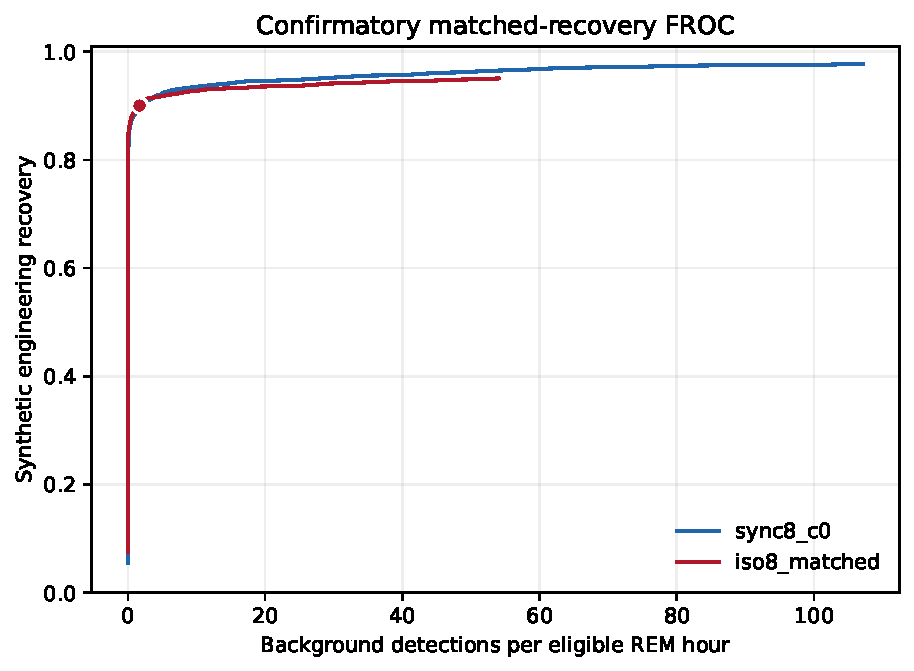
\includegraphics[width=0.78\textwidth]{../outputs/ocular-code-confirmatory/sc-analysis/confirmatory_froc.pdf}
\caption{SC matched-recovery FROC curves. The filled markers show the prespecified 90\% operating point. Lower rates indicate fewer accidental matches. The curves cross at high recovery, but the 95\% point was descriptive after failure of the primary gate.}
\label{fig:froc}
\end{figure*}

\subsection{External sleep-telemetry test}

The ST placebo cohort contained 22 nights from 22 participants, 34.237 eligible REM hours, and 440 paired injections per code. At exactly 95\% recovery, the rhythmic code produced 8.996 events per hour and the control produced 9.376. The difference was $-0.380$ per hour, with a 95\% interval from $-10.523$ to 12.394. The rate ratio was 0.960. Both external replication rules failed.

Applying the SC 95\% thresholds directly to ST gave a different impression (Table~\ref{tab:transport}). The rhythmic rate was then 7.214 per hour and the control rate was 16.795. However, recovery was 94.32\% for the rhythmic code and 95.68\% for the control. Once both thresholds were reselected within ST to give exactly 95\% recovery, the large apparent specificity advantage nearly disappeared.

\begin{table}[t]
\centering
\caption{Threshold transport to ST placebo. Fixed SC thresholds changed both collision rate and recovery. Rematching restored equal recovery.}
\label{tab:transport}
\small
\begin{tabular}{lrr}
\toprule
Condition & \texttt{sync8\_c0} & \texttt{iso8} \\
\midrule
Fixed SC threshold & 0.5434 & 0.4521 \\
ST recovery & 94.32\% & 95.68\% \\
ST events/h & 7.214 & 16.795 \\
\addlinespace
Rematched ST threshold & 0.5329 & 0.4909 \\
ST recovery & 95.00\% & 95.00\% \\
ST events/h & 8.996 & 9.376 \\
\bottomrule
\end{tabular}
\end{table}

\section{Discussion}

The rhythmic code did not show a robust background-resistance advantage at equal synthetic recovery. The SC point estimate at 90\% favored the isochronous control slightly. The external ST estimate at 95\% favored the rhythmic code slightly, but the interval was wide and the prespecified replication rules failed. These results do not establish equivalence. They do show that the available data do not justify advancing this code as generally superior.

The more useful finding concerns evaluation. A fixed detector score is not a fixed sensitivity when the acquisition cohort changes. In ST, transporting two SC thresholds produced unequal recovery and an apparently large rate difference. Comparing the codes at equal recovery reduced that difference from 9.580 to 0.380 events per hour. An asynchronous physiological interface should therefore report a continuous-time FROC curve, false activations per unit exposure, and recovery at every claimed operating point. Window accuracy alone can hide the operational false-alarm burden.

The benchmark also separates code recognition from participant behavior. Synthetic injections measure whether the software can recover a perturbed waveform in real background noise. They do not measure whether a lucid dreamer can execute the pattern, remember the instruction, or remain asleep. Visible dream signals can differ from the intended or reported sequence \citep{oudiette2018}, and learned multi-direction EOG gestures introduce further motor and classifier demands \citep{amo2025}. Human production must therefore be tested prospectively with intentional signals and independently labeled opportunities.

The study has four main limitations. First, the source recordings contain spontaneous REM without instructed code production, so no human sensitivity estimate is available. Second, synthetic perturbations approximate only a limited family of timing and amplitude variation. Third, the ST cohort is small and gives imprecise participant-level intervals. Fourth, Sleep-EDF was not collected for lucid dreaming or real-time interaction. Current interactive-dreaming studies demonstrate that some sleepers can process questions and answer during REM \citep{konkoly2021,turker2023}, but that fact does not guarantee reliable asynchronous activation.

The next empirical step should be a prospective human study with a frozen detector. Participants would attempt both codes in randomized order during verified lucid REM and during waking calibration. The primary outcomes should be detected intentional emissions per instructed opportunity and false activations per REM hour outside response windows. Only after ordinary-channel reliability is established would it make sense to design any blinded test of anomalous information transfer. The present data contain no such test and no evidence for psi.

\section{Conclusion}

Across two independent Sleep-EDF cohorts, a rhythmic eight-interval ocular code did not produce a reproducible reduction in spontaneous REM collisions when compared with an equal-duration isochronous code at matched synthetic recovery. The main contribution is methodological: portable ocular interfaces require exposure-normalized continuous scanning and equal-sensitivity comparison across corpora. Fixed score thresholds can create a misleading specificity advantage when detector-score distributions shift.

\section*{Data and code availability}

All protocols, manifests, analysis code, machine-readable result tables, and figure sources are available in the \href{https://github.com/asim-v/rem-ocular-code-collision-benchmark}{public GitHub repository}. Sleep-EDF Expanded is available from \href{https://physionet.org/content/sleep-edfx/1.0.0/}{PhysioNet}. Raw physiological files are not redistributed by the repository.

\section*{Ethics statement}

This computational study reanalyzed deidentified public recordings and did not recruit participants or collect new human data.

\section*{Competing interests}

The author declares no competing interests.

\small
\bibliographystyle{unsrtnat}
\bibliography{references}

\end{document}
